\documentclass{article}
\usepackage{amsmath,amssymb,amsfonts,amsthm, dsfont, color}
\usepackage{bm}
\usepackage{bbm}
\usepackage{amsfonts}
\usepackage{tikz}
\usepackage{pgfplots}
\usepackage{colortbl}
\usetikzlibrary{external}
\usetikzlibrary{shapes.misc, positioning}
\usetikzlibrary{decorations.pathreplacing}
\usetikzlibrary{arrows.meta, shapes,patterns.meta}

\tikzset{
  block/.style    = {draw, thick, rectangle, minimum width = 2em},
sblock/.style      = {draw, thick, rectangle, minimum height = 2em,
minimum width = 2em}, 
}
        
\definecolor{embed}{HTML}{AEF78E}
\definecolor{attn}{HTML}{f9e3ae}
\definecolor{ff}{HTML}{90F3FF}
\definecolor{lin}{HTML}{E15CEC}
\definecolor{mask1}{HTML}{4D4847}
\definecolor{mask2}{HTML}{30343F}

\newcommand{\vect}[1]{\boldsymbol{#1}}
\newcommand{\bx}{\vect{x}}
\newcommand{\by}{\vect{y}}
\newcommand{\bz}{\vect{z}}
\newcommand{\logit}{\mathrm{logit}}
\newcommand{\btheta}{\vect{\theta}}
\newcommand{\thetabar}{\bar{\btheta}}

\tikzexternalize

\begin{document}
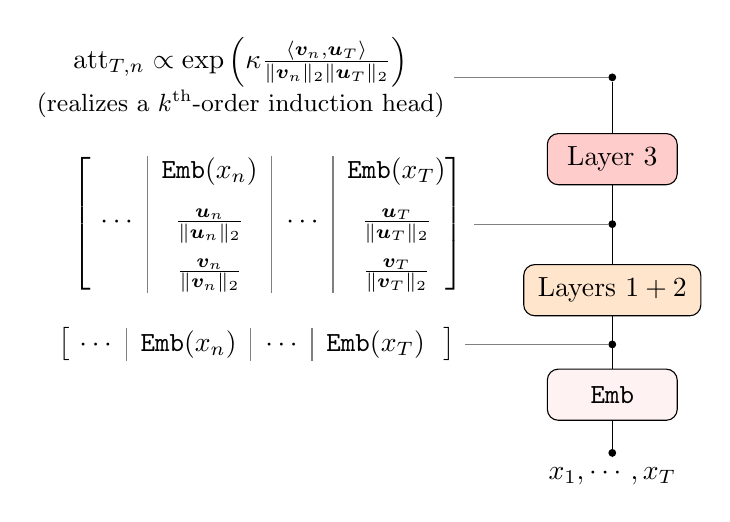
\begin{tikzpicture}[
    node distance=2cm,
    startstop/.style={rectangle, rounded corners, minimum width=1.65cm, minimum height=0.65cm,text centered, draw=black},
    process/.style={rectangle, minimum width=3cm, minimum height=1cm, text centered, draw=black, fill=orange!30},
    io/.style={trapezium, trapezium left angle=70, trapezium right angle=110, minimum width=3cm, minimum height=1cm, text centered, draw=black, fill=blue!30},
    decision/.style={diamond, minimum width=3cm, minimum height=1cm, text centered, draw=black, fill=green!30},
    every text node part/.style={align=center},
    cross/.style={path picture={ 
  \draw[black]
(path picture bounding box.east) -- (path picture bounding box.west) (path picture bounding box.south) -- (path picture bounding box.north);
}}
    ]

    \node (l1) [startstop, fill=orange!20,  minimum width=2.25cm]      {Layers $1+2$};
    \node (l2out) [circle,fill,inner sep=1pt, above = 0.45cm of l1] {}; \node (l2outlabel) [left = 1.7cm of l2out] {$\arrayrulecolor{gray}\left[\begin{array}{@{}c|c|c|c@{}}
& \texttt{Emb} (x_n) & & \texttt{Emb} (x_T) \\[6pt] \ \cdots & \frac{\bm{u}_{n}}{\| \bm{u}_{n} \|_2} & \cdots & \frac{\bm{u}_{T}}{\| \bm{u}_{T} \|_2} \\[6pt] & \frac{\bm{v}_{n}}{\| \bm{v}_{n} \|_2} & & \frac{\bm{v}_T}{\| \bm{v}_T \|_2}
\end{array}\right]$};
    \node (l3) [startstop, fill=red!20, above = 1cm of l1]      {Layer $3$};
    \node (l1in) [circle,fill,inner sep=1pt, below = 0.3cm of l1]  {};
    \node (l1inlabel) [left = 1.82cm of l1in] {$\arrayrulecolor{gray}\left[\begin{array}{@{}c|c|c|c@{}}
\ \cdots & \texttt{Emb} (x_n) & \cdots & \texttt{Emb} (x_T) \ \
\end{array}\right]$};
    % \node (l3out) [circle,fill,inner sep=1pt, left = 0.75cm of l1]  {}     node[below = 0.25cm of l1in] {$e_{x_n}$};
    \node (l3out) [circle, fill, inner sep=1pt, above = 0.65cm of l3] {};
    \node (l3outlabel) [left = 1.95cm of l3out] {$\operatorname{att}_{T,n} \propto \exp \left( \kappa \frac{\langle \bm{v}_n, \bm{u}_T \rangle}{\| \bm{v}_n \|_2 \| \bm{u}_T \|_2} \right)$ \\ {\small(realizes a $k^{\text{th}}$-order induction head)}};
    \node (emb) [startstop, below = 0.25cm of l1in, fill=pink!20] {$\texttt{Emb}$};
    \node (l0in) [circle,fill,inner sep=1pt, below = 0.35cm of emb] {} node [below = 0cm of l0in] {$x_1,\cdots,x_T$};
    

    \draw[-,color=gray] (l1in.west) -| (l1inlabel.east);
    \draw[-,color=gray] (l2out.west) -| (l2outlabel.east);
    \draw[-,color=gray] (l3out.west) -| (l3outlabel.east);
    \draw[-] (l1in.south) -| (l1.south);
    \draw[-] (emb.north) -| (l1in.south);
    \draw[-] (l1.north) -| (l3.south);
    \draw[-] (l3.north) -| (l3out.south);
    \draw[-] (l0in.south) -| (emb.south);
  \end{tikzpicture}
\end{document}